\documentclass[%
autoref,     % тип документа
href,        % использовать пакет hyperref для создания гиперссылок
facsimile,   % отображать факсимиле диссертанта и ученого секретаря
colorlinks,  % цветные гиперссылки
%fixint,     % отключить прямые знаки интегралов
%times,      % шрифт Times как основной
%classified, % гриф секретности
]{disser}

\usepackage[
  a4paper, mag=1000,
  left=2.5cm, right=1cm, top=2cm, bottom=2cm, headsep=0.7cm, footskip=1cm
]{geometry}
\usepackage[T2A]{fontenc}
\usepackage[utf8]{inputenc}
\usepackage[english,russian]{babel}
\usepackage{tabularx}
\usepackage{csquotes}
\ifpdf\usepackage{epstopdf}\fi

\usepackage[style=gost-numeric,
  backend=biber,
  language=auto,
  hyperref=auto,
  autolang=other,
  defernumbers=true,
  sorting=nyt
]{biblatex}

\addbibresource{thesis.bib}

% Номера страниц снизу и по центру
\pagestyle{footcenter}
\chapterpagestyle{footcenter}

% Точка с запятой в качестве разделителя между номерами цитирований
%\setcitestyle{semicolon}

% Путь к файлам с иллюстрациями
\graphicspath{{fig/}}

\begin{document}
% Включение файла с общим текстом диссертации и автореферата
% (текст титульного листа и характеристика работы).
% Общие поля титульного листа диссертации и автореферата
\institution{Название организации}

\topic{Тема диссертации}

\author{Скурыдина Алия Фиргатовна}

\specnum{01.01.07}
\spec{Вычислительная математика}
%\specsndnum{01.04.07}
%\specsnd{Физика конденсированного состояния}

\sa{Акимова Елена Николаевна}
\sastatus{д.~ф.-м.~н., доц.}
%\sasnd{ФИО второго руководителя}
%\sasndstatus{к.~ф.-м.~н., проф.}

%\scon{ФИО консультанта}
%\sconstatus{д.~ф.-м.~н., проф.}
%\sconsnd{ФИО второго консультанта}
%\sconsndstatus{д.~ф.-м.~н., проф.}

\city{Екатеринбург}
\date{\number\year}

% Общие разделы автореферата и диссертации
\mkcommonsect{actuality}{Актуальность темы исследования.}{%
Построение итеративно регуляризованных алгоритмов востребовано для решения широкого круга прикладных некорректно поставленных задач. Так, решение структурных обратных задач гравиметрии и магнитометрии сводится к решению нелинейных интегральных уравнений Урысона первого рода. После дискретизации операторное уравнение сводится к системе нелинейных уравнений с большим числом неизвестных, поэтому есть необходимость в параллелизации алгоритмов для многопроцессорных и многоядерных вычислительных систем с целью уменьшения времени счета. 
}

\mkcommonsect{development}{Степень разработанности темы исследования.}{
Ж. Адамар в 1902 г.~\cite{Hadamar1902} впервые определил условия корректности задачи математической физики. Задачи, не отвечающие этим условиям, то есть некорректные,  Ж. Адамар считал лишенными физического смысла. В течение многих лет обратные задачи решались методом подбора, например, в геофизике, сравнивая вычисленное физическое поле модели с наблюденным. Однако со временем, это мнение претерпело изменения.

Первой работой по теории некорректных задач считается известная работа академика А.Н. Тихонова 1943 г.~\cite{Tikh1943}, в которой он доказал устойчивость некоторых обратных задач при условии принадлежности решения компактному множеству. Также в этой работе он решил одну из актуальных обратных задач разведочной геофизики. В дальнейшем теория некорректных задач оформилась в самостоятельный раздел современной математики. В конце 50-х годов и начале 60-х годов появились работы, посвященные решению некоторых некорректных задач с помощью идей регуляризации, выдающихся отечественных ученых: А.Н. Тихонова, М.М. Лаврентьева, В.К. Иванова. Их исследования в этой области положили начало трем научным школам:  Московской, Сибирской и Уральской.
Началось исследование устойчивых методов решения некорректно-поставленных задач, представляющих собой одно из наиболее актуальных проблем современной математической науки.

В большом цикле работ, выполненных начиная с 1963 года, А.Н. Тихонов сформулировал принцип устойчивого решения некорректно-поставленных задач, ввел понятие регуляризирующего оператора и предложил ряд эффективных методов построения таких операторов, легко реализуемых на ЭВМ ~\cite{Tikh1963_1, Tikh1963_2, TikhGlas1965, TikhArs1986}. Метод, получивший название "метод регуляризации А.Н. Тихонова"\, был применен для решения большого количества как фундаментальных математических, так и актуальных прикладных задач. В частности, тихоновским методом регуляризации были решены задача об отыскании решения интегрального и операторного уравнения первого рода, обратные задачи теории потенциала и теплопроводности. 

Наряду с Тихоновым, М.М. Лаврентьев изучал методы регуляризации. Ему принадлежит идея замены исходного уравнения близким ему, в некотором смысле, уравнением, для которого задача нахождения решения устойчива к малым изменениям правой части и разрешима для любой правой части ~\cite{Lavr1962}. Были доказаны теоремы сходимости регуляризованного решения к точному ~\cite{Lavr1956}. Основополагающие  результаты  для  интегральных  уравнений  Фредгольма  первого  рода  получены  в  ~\cite{Lavr1959, Lavr1963, LavrVas1966, LavrRomShi1980},  где  для  решения  линейных  интегральных  уравнений  Фредгольма  первого  рода  построены  регуляризирующие  операторы  по  М.М. Лаврентьеву. 

В работах Иванова, выполненных в 1960--1970-е гг., было введено понятие квазирешения ~\cite{Iv1962_2, Iv1963}, были заложены также основы двусторонних оценок регуляризующих алгоритмов ~\cite{Iv1966}, установлены связи между вариационными методами регуляризации, развит единый подход к трактовке линейных некорректных задач в топологических пространствах ~\cite{Iv1967}. 

Однако не все некорректные задачи возможно регуляризовать. Так, российский математик Л.Д. Менихес ~\cite{Menih1978} привел пример интегрального оператора с непрерывным замкнутым ядром, действующего из пространства \( C[0,1] \) в \( L_2[0,1] \), обратная задача для которого нерегуляризуема. Проблемам регуляризуемости также посвящены работы Ю.И. Петунина и А.Н. Пличко ~\cite{PetPlich1980}.

Для построения регуляризующих алгоритмов для решения прикладных задач требуется использовать дополнительную информацию о свойствах искомого решения, заданную в виде равенств и неравенств, характеристик решения, например, свойствами гладкости, естественно вытекающих из физической сущности задачи. Получило развитие построение регуляризующих алгоритмов вариационными методами. А.Б. Бакушинский, Б.Т. Поляк сформулировали общие принципы построения регуляризующих алгоритмов в банаховых пространствах \cite{BakPol1974}. Метод обобщенной невязки был предложен А.В. Гончарским, А.С. Леоновым, А.Г. Яголой \cite{GonLeoYag1973}.  Монография А.Б. Бакушинского, А.В. Гончарского \cite{BakGon1989} посвящена итеративной регуляризации вариационных неравенств с монотонными операторами, которые единообразно описывают многие постановки задач с априорной информацией. В работе \cite{Bak1992} А.Б. Бакушинский предложил модификацию метода Гаусса -- Ньютона в духе итеративной регуляризации и исследовал его на сходимость. Метод
Гаусса -- Ньютона был также исследован в работах B. Blaschke, A. Neubauer, O. Scherzer, B. Kaltenbacher, A.G.Ramm \cite{BlaNeuSch1997,KalNeuRam2002}.

Методам решения операторных уравнений первого рода посвящены работы В.П. Тананы~\cite{Tan1977, Tan1997} и монография \cite{Tan1981}. Им был введен метод $L$-регуляризации, представляющий собой разновидность метода Тихонова, расширивший класс регуляризуемых задач \cite{Tan2003_1,Tan2003_2}.

Регуляризующие алгоритмы в пространствах функций ограниченной вариации были впервые предложены М.Г. Дмитриевым, В.С. Полещуком \cite{DmiPol1972}, И.Ф. Дорофеевым \cite{Dor1979}. Далее в работах А.В. Гончарского и В.В. Степанова \cite{GonSte1979} А.Л. Агеева \cite{Ag1980} была доказана равномерная сходимость приближенных решений. Подход, изложенный в \cite{TikhGonSteYag1990} основан на идее двухэтапного алгоритма: построении приближенного решения  исходного операторного уравнения из условия минимизации регуляризованной невязки на априорном множестве, где привлекается информация о неотрицательности, монотонности и выпуклости решения: $$min\{\| A(u)-f_\delta\| ^2 + \alpha \Omega(u): u\in\Omega, \|f-f_\delta\|\le\delta \},$$ 
где $A$ --- оператор задачи, $f$ --- правая часть без шума, $f_\delta$ --- возмущенная правая часть, $\delta$ --- уровень шума, $\alpha$ --- параметр регуляризации. 

На втором этапе для решения корректно поставленной экстремальной задачи применяются методы градиентного типа, линеаризованные методы, или алгоритмы, специально ориентированные на определенный класс априорных ограничений.

Для решения систем нелинейных уравнений предложены методы в работах Л.В. Канторовича \cite{Kan1947}, Б.Т. Поляка \cite{Pol1969}, J. M. Ortega и W. C. Rheinboldt \cite{OrtRhe1970}, A. Neubauer, O. Scherzer \cite{NeuSch1995, Sch1995}, M.J.D. Powell \cite{Pow1970}, J.E.Dennis, R.B. Schnabel, P.D. Frank \cite{DenSchn1996}, C.T. Kelley \cite{Kel1995}, R.B. Schnabel и P.D. Frank \cite{SchnFra1983} для решения систем уравнений с сингулярной или плохо обусловленной матрицей Якоби, J.C. Gilbert, J. Nocedal, S.J. Wright \cite{GilNoc1991, NocWri2006}. Термин $\alpha$-процессы, характеризующий класс нелинейных итерационных методов (где оператор шага нелинеен) для решения линейного уравнения с ограниченным самосопряженным положительно полуопределенным оператором был введен в монографии М.А. Красносельского, Г.М. Вайникко, П.П. Забрейко \cite{KraVayZab1969}. Сходимость и устойчивость методов наискорейшего спуска и минимальной ошибки исследовалась авторами A. Neubauer, O. Scherzer в \cite{NeuSch1995}.

L. Landweber в статье \cite{Lan1951} 1951 г. предложил метод для решения линейных интегральных уравнений Фредгольма I рода. В дальнейшем авторы M. Hanke, A. Neubauer и O. Scherzer \cite{HanNeuSch1995,Neu2000,NeuSch1995} применили метод Ландвебера для решения нелинейных нерегулярных уравнений, доказали теоремы о сходимости и исследовали скорость сходимости метода. Градиентные методы с применением метода Ландвебера исследовались М.Ю. Кокуриным в работах \cite{Kok2010_1,Kok2010_2}.

В работах \cite{Han1997,Han2010} M. Hanke предложил новую схему метода Левенберга -- Марквардта для решения некорректных задач на примере задачи фильтрации.

В.В. Васиным предложен подход к решению задач с априорной информацией в работах ~\cite{Vas1982, Vas1988} и в монографиях ~\cite{VasAge1993, VasEre2005}, основанный на применении фейеровских отображений для учета априорных ограничений в форме выпуклых неравенств. Термин <<фейеровское отображение>> введен Ереминым в работах ~\cite{Ere1965, Ere1966, Ere1968} в честь венгерского математика Фейера. Отображения, обладающие свойством фейеровости, позволяют строить итерационные процессы с учетом априорных ограничений достаточно общего вида и, в отличие от метрической проекции, допускают эффективную реализацию. На основе $\alpha$-процессов были предложены регуляризованные методы решения линейных операторных уравнений Фредгольма $I$ рода, возникающих, например, при решении линейных обратных задач гравиметрии. Также Васин доказал сильную сходимость метода Левенберга -- Марквардта и его модифицированного варианта для решения регуляризованного по Тихонову нелинейного уравнения. Были приведены численные эксперименты для нелинейной обратной задачи гравиметрии в работах В.В. Васина и Г.Я. Пересторониной~\cite{VasPer2011}, В.В. Васина ~\cite{Vas2012}. Они показали, что основной процесс Левенберга -- Марквардта существенно превосходит по точности модифицированный вариант и не требует жестких условий на начальное приближение, но обладает большей вычислительной сложностью, и, следовательно, требует больших затрат машинного времени.

При исследовании методов решения некорректных задач важное место занимает оценка погрешности регуляризованного решения по отношению к точному решению. Для уравнения с монотонным оператором исследовался метод Лаврентьева U. Tautenhahn \cite{Tau2002,Tau2004}, стратегия выбора параметра регуляризации по Тихонову исследовался авторами Q. Jin Zong-Yi Hou, O. Scherzer, H. W. Engl и K. Kunisch \cite{JinZon1997,JinZon1999,SchEngKun1993}. В.П. Тананой была доказана сходимость решения $L$-регуляризованной вариационной задачи к решению исходного операторного уравнения $I$ рода, продемонстрировав на примере двумерной обратной задачи гравиметрии \cite{Tan2003_2}.
}

\mkcommonsect{objective}{Цели и задачи диссертационной работы:}{%
построить новые методы решения нелинейных операторных уравнений первого рода в гильбертовом пространстве, исследовать их сходимость. Предложить методы решения обратной задачи гравиметрии, использующие особенности физической модели.
%
%Для достижения поставленных целей были решены следующие задачи:
%\begin{itemize}
%	\item для нелинейного уравнения с монотонным оператором доказаны теоремы сходимости для регуляризованного метода Гаусса -- Ньютона, доказана сильная фейеровость итерационных процессов;
%	\item построены регуляризованные методы градиентного типа, названные нелинейными аналогами $\alpha$-процессов, для нелинейного уравнения с монотонным оператором доказаны теоремы сходимости для них, доказана сильная фейеровость итерационных процессов;
%	\item для задачи с немонотонным оператором с производной, имеющей неотрицательный спектр, доказаны теоремы сходимости методов Ньютона, нелинейных $\alpha$-процессов и их модифицированных вариантов;
%	\item предложена вычислительная оптимизация метода Ньютона и его модифицированного варианта при решении задач с матрицей производной, близкой к ленточной;
%	\item lля решения систем нелинейных интегральных уравнений  с ядром оператора структурной обратной задачи гравиметрии в двуслойной среде предложен покомпонентный метод, основанный на методе Ньютона;
%	\item для решения систем нелинейных уравнений  структурных обратных задач гравиметрии в многослойной среде предложен подход на основе метода Левенберга -- Марквардта --- покомпонентный метод типа Левенберга --- Марквардта;
%	\item проведены численные эксперименты, интерпретированы результаты.
%\end{itemize}
}

\mkcommonsect{novelty}{Научная новизна.}{%
Результаты, полученные в диссертационной работе, являются новыми и состоят в следующем:

	в рамках двухэтапного метода построения регуляризующего алгоритма обоснованы сходимость метод Ньютона и нелинейные аналоги альфа-процессов: метод минимальной ошибки (ММО), метод наискорейшего спуска (МНС) и метод минимальных невязок (ММН). Также установлена сходимость модифицированных вариантов методов ММО, МНС, ММН, когда производная оператора вычисляется в начальной точке итераций. Рассмотрены два случая: оператор задачи является монотонным, либо оператор является конечномерным и его производная имеет неотрицательный спектр.
	
	Для решения систем нелинейных интегральных уравнений  с ядром оператора структурной обратной задачи гравиметрии в двуслойной среде предложен покомпонентный метод, основанный на методе Ньютона. 
	Предложена вычислительная оптимизация метода Ньютона и его модифицированного варианта в виде перехода от плотно заполненной матрицы производной оператора к ленточной в силу особенности строения ядер интегральных операторов задач грави- магнитометрии.
	Для решения систем нелинейных уравнений  структурных обратных задач гравиметрии в многослойной среде предложен подход на основе метода Левенберга-Марквардта – покомпонентный метод типа Левенберга-Марквардта.

}

\mkcommonsect{value}{Теоретическая и практическая значимость.}{%
Результаты, изложенные в диссертации, могут быть использованы для решения нелинейных операторных уравнений, в частности, задач гравиметрии и магнитометрии.
}

\mkcommonsect{methods}{Методология и методы исследования.}{%
Текст о методах исследования.
}

\mkcommonsect{results}{Положения, выносимые на защиту:}{%
1. Сформулированы и доказаны теоремы, устанавливающие сильную фейеровость оператора шага итераций методов:
	\begin{itemize}
		\item 	метод Ньютона;
		\item	метод минимальной ошибки и его модифицированный вариант;
		\item	метод наискорейшего спуска и его модифицированный вариант;
		\item	метод минимальных невязок и его модифицированный вариант.
	\end{itemize}
	
	Доказана сильная фейеровость оператора шага итераций данных методов в случае монотонного оператора задачи и в случае конечномерного оператора с производной, имеющей неотрицательный спектр. Доказывается линейная скорость сходимости итерационных процессов.
	
	2. Предложена вычислительная оптимизация метода Ньютона, которая в задачах гравиметрии и магнитометрии обеспечивает более высокую точность численного решения, а также уменьшает время счета программ.
	
	3. Предложены покомпонентные методы:
		\begin{itemize}
			\item покомпонентный основанный на методе Ньютона для решения нелинейного интегрального уравнения в задаче гравиметрии в двухслойной среде;
			\item покомпонентный метод типа Левенберга-Марквардта для решения систем нелинейных уравнений  структурных обратных задач гравиметрии в многослойной среде.
		\end{itemize} Данные методы обладает меньшей вычислительной сложностью в отличие от классических методов Ньютона и Левенберга-Марквардта.
		
Вычислительные эксперименты показывают, что предложенные метод позволяют существенно уменьшить вычислительную сложность задачи и являются экономичными по потреблению памяти ЭВМ.
		
		4. Проведены численные эксперименты для модельных и квазиреальных геофизических данных, разработан комплекс параллельных программ для многоядерных и графических процессоров с использованием технологий OpenMP, CUDA. 
}

\mkcommonsect{approbation}{Степень достоверности и апробация результатов.}{%
Основные результаты по материалам диссертационной работы докладывались на конференциях:

1. XIV и XV Уральская молодежная научная школа по геофизике (Пермь, 2013 г., Екатеринбург 2014 г.);

2. Международная коференция "Параллельные вычислительные технологии" (Ростов-на-Дону, 2014 г., Екатеринбург, 2015 г., Казань, 2017 г.);

3. Международная конференция «Геоинформатика: теоретические и прикладные аспекты» (Киев 2014, 2015, 2016 г.)

4. Международная конференция "Актуальные проблемы вычислительной и прикладной математики" (Новосибирск, 2014 г.)

5. Международный научный семинар по обратным и некорректно поставленным задачам (Москва, 2015 г.)
}

\mkcommonsect{pub}{Публикации.}{%
Материалы диссертации опубликованы в $13$ печатных работах, из них $4$
статей в рецензируемых журналах~\cite{Ivanov_1999_Journal_17_173,
Petrov_2001_Journal_23_12321,Sidorov_2002_Journal_32_1531}, $2$ статей в
сборниках трудов конференций и $7$ тезисов докладов.
}

\mkcommonsect{contrib}{Личный вклад автора.}{%
Результаты, представленные в данной работе, получены автором лично.
}

\mkcommonsect{struct}{Структура и объем диссертации.}{%
Диссертация состоит из введения, обзора литературы, $3$ глав, заключения и библиографии.
Общий объем диссертации $\pageref{LastPage}$ страниц, из них $p_1$ страницы текста, включая $n$ рисунков, $m$ таблиц.
Библиография включает $B$ наименований на $p_2$ страницах.
}


% номер копии для грифа секретности
%\copynum{1}
% класс доступа
%\classlabel{Для служебного пользования}

\title{АВТОРЕФЕРАТ\\
диссертации на соискание ученой степени\\
кандидата физико-математических наук}

\maketitle

% Внутренняя сторона обложки
\thispagestyle{empty}
\vspace*{-2cm}
\noindent
\small
\begin{center}
Работа выполнена в \emph{Федеральном государственном бюджетном учреждении науки Институт математики и механики им. Н. Н. Красовского Уральского отделения Российской академии наук}.
\end{center}
\vskip1ex
\begin{tabularx}{\linewidth}{lp{1cm}X}
Научный руководитель:  & & \emph{доктор физико-математических наук}, \\
                       & & \emph{доцент Акимова Елена Николаевна}
\\
Официальные оппоненты: & & \emph{доктор физико-математических наук}, \\
                       & & \emph{профессор, главный научный сотрудник кафедры Системного программирования ФГАОУ ВО <<Южно-Уральский государственный
                       	университет (национальный исследовательский
                       	университет)>> (г. Челябинск)}, \\
                       & & \emph{Танана Виталий Павлович}\\
                       & & \emph{доктор физико-математических наук}, \\
                       & & \emph{профессор, профессор кафедры математики физического факультета ФГБОУ ВО <<Московский государственный университет имени М. В. Ломоносова>>}, \\
                       & & \emph{Ягола Анатолий Григорьевич}
\\
Ведущая организация:   & & \emph{ФГАОУ ВО <<Казанский (Приволжский) федеральный университет>>}\\
\end{tabularx}

\vskip2ex\noindent
Защита состоится \datefield{} в \rule[0pt]{1cm}{0.5pt} часов
на заседании диссертационного совета \emph{Д 004.006.04} при \emph{ФГБУН Институт математики и механики им. Н. Н. Красовского УрО РАН} по адресу:
\emph{620990, Екатеринбург, ул. Софьи Ковалевской, 16, актовый зал}

\vskip1ex\noindent
С диссертацией можно ознакомиться в библиотеке
\emph{ФГБУН Институт математики и механики им. Н. Н. Красовского УрО РАН}.

\vskip1ex\noindent
Автореферат разослан \datefield{}

\vskip2ex\noindent
Отзывы и замечания по автореферату в двух экземплярах, заверенные
печатью, просьба высылать по вышеуказанному адресу на имя ученого секретаря
диссертационного совета.

\vfill\noindent
\begin{minipage}[b]{0.4\linewidth}
  Ученый секретарь\\
  диссертационного совета,\\
  \emph{доктор физ.-мат. наук}, \emph{с.н.с.}
\end{minipage}
\hfill
% вставка файла, содержащего факсимиле ученого секретаря
\makeatletter
\ifDis@facsimile
  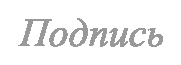
\includegraphics[width=3cm]{sec-facsimile}\hfill
\fi%
\makeatother%
\emph{Скарин В. Д.}

\clearpage

\normalsize
\nsection{Общая характеристика работы}

% Актуальность работы
\actualitysection
\actualitytext

% Степень разработанности темы исследования
%\developmentsection
%\developmenttext

% Цели и задачи диссертационной работы
\objectivesection
\objectivetext

% Научная новизна
\noveltysection
\noveltytext

% Теоретическая и практическая значимость
\valuesection
\valuetext

% Методология и методы исследования
%\methodssection
%\methodstext

% Положения, выносимые на защиту
\resultssection
\resultstext

% Степень достоверности и апробация результатов
\approbationsection
\approbationtext

% Публикации
\pubsection
\pubtext

% Личный вклад автора
\contribsection
\contribtext

% Структура и объем диссертации
\structsection
\structtext

\nsection{Содержание работы}

\textbf{Во Введении} обоснована актуальность диссертационной работы, сформулирована цель и аргументирована научная новизна исследований, показана практическая значимость полученных результатов, представлены выносимые на защиту научные положения.

\textbf{В первой главе} ...

Содержание первой главы.

Результаты первой главы опубликованы в работе~\cite{VasSkur2017}.

\textbf{Во второй главе} ...

Содержание второй главы.

Результаты второй главы опубликованы в работе~\cite{VasSkur2017}.

\textbf{В третьей главе} ...

Содержание третьей главы.

Результаты третьей главы опубликованы в работах~\cite{AkSkur2014}, \cite{AkSkur2015}, \cite{AkSkur2016}, \cite{Skur2017_2}.

\textbf{В Заключении}

\nsection{Основные результаты диссертации}

1. Для нелинейного уравнения с монотонным оператором доказаны теоремы сходимости для регуляризованного метода Ньютона, построены регуляризованные методы градиентного типа для решения нелинейного уравнения с монотонным оператором --- метод минимальной ошибки, метод наискорейшего спуска, метод минимальных невязок, названные нелинейными аналогами $\alpha$-процессов, доказаны теоремы сходимости для них, доказана сильная фейеровость итерационных процессов.

Для задачи с немонотонным оператором, производная которого имеет неотрицательный спектр, доказаны теоремы сходимости методов Ньютона, нелинейных $\alpha$-процессов и их модифицированных вариантов. 

2. Для решения систем нелинейных интегральных уравнений  с ядром оператора структурной обратной задачи гравиметрии для модели двухслойной среды предложен покомпонентный метод, основанный на методе Ньютона. Предложена вычислительная оптимизация метода Ньютона и его модифицированного варианта при решении задач с матрицей производной, близкой к ленточной; на примере решения обратной задачи гравиметрии продемонстрирована вычислительная экономичность модификации. Для решения систем нелинейных уравнений  структурных обратных задач гравиметрии для моделей двухслойной и многослойной сред предложен подход на основе метода Левенберга -- Марквардта --- покомпонентный метод типа Левенберга -- Марквардта.

3. Разработан комплекс параллельных программ, с использованием многоядерных процессоров для всех предложенных методов и с вычислением на графических процессорах (видеокартах) для покомпонентных методов и метода Ньютона и модифицированного варианта.

В дальнейшей научной работе автора предполагается исследование на сходимость покомпонентных методов типа Ньютона и Левенберга -- Марквардта.

% ----------------------------------------------------------------
\printbibheading[title={Основные публикации по теме диссертации}]
%Если не работает - коммент-анкоммент, все будет чики-чики
\printbibliography[
heading=subbibliography,
keyword=hac,
title={Статьи в изданиях из перечня ВАК, SCOPUS}
]

\printbibliography[
heading=subbibliography,
keyword=nohac,
title={Другие публикации}
]
%\printbibliography[notkeyword=own,title={Цитированная литература}]

% ----------------------------------------------------------------
% Выходные данные
\clearpage
\thispagestyle{empty}
\normalfont\selectfont
\vspace*{2cm}
\begin{center}
\textit{Научное издание}\\
\vskip 2cm
\makeatletter
\@author
\vskip 1.5cm
\@title{} на тему:\\
\@topic\\
\makeatother
\end{center}
\vfill
Подписано в печать~25.01.2011.
Формат~$60 \times 90$~1/16.
Тираж~100~экз.
Заказ~256.\\[2ex]
\noindent
Санкт-Петербургская издательская фирма <<Наука>> РАН.
199034, Санкт-Петербург, Менделеевская линия, 1,
\href{http://www.naukaspb.spb.ru}{http://www.naukaspb.spb.ru}

\end{document}
